% =====================================================================
%  Data Mining · SGH · SMMD-ADA   —   Block 3 slide deck
%  Template: Frankfurt + seahorse + miniframes (same as course template)
%
%  Compilation:
%    pdflatex block3.tex   (run twice for the section headline)
%
%  Figures: regenerate with   uv run python lecture_3/make_figures.py
%
%  Speaker-notes display modes (uncomment one):
%    \setbeameroption{hide notes}                          % slides only
%    \setbeameroption{show notes}                          % slides + note pages
%    \setbeameroption{show notes on second screen=right}   % presenter mode
%    \setbeameroption{show only notes}                     % notes printout
% =====================================================================
\documentclass[10pt,aspectratio=169]{beamer}

\usepackage[utf8]{inputenc}
\usepackage[T1]{fontenc}
\usepackage{booktabs}
\usepackage{array}
\usepackage{multirow}
\usepackage{amsmath,amssymb}
\usepackage{graphicx}
\usepackage{xcolor}
\usepackage{tikz}
\usetikzlibrary{arrows.meta,positioning,shapes.geometric}

% - Theme -
\usetheme{Frankfurt}
\usecolortheme{seahorse}
\useoutertheme{miniframes}
\setbeamertemplate{navigation symbols}{}
\setbeamertemplate{footline}[frame number]

% - Speaker notes -
\setbeameroption{hide notes}
% \setbeameroption{show notes on second screen=right}

% - Colours for figures -
\definecolor{sghblue}{RGB}{0,51,102}

% - Metadata -
\title[Data Mining]{Data Mining}
\subtitle{Block 3 - Trees, ensembles \& honest evaluation}
\author{Daniel Wlazło}
\institute{SGH Warsaw School of Economics - SMMD-ADA}
\date{20 October 2026}

\begin{document}

% ============================================================
\begin{frame}[plain]
  \begin{center}
    \vspace{1cm}
    {\LARGE\textbf{Data Mining}}\\[0.5cm]
    {\large Block 3 - Trees, ensembles \& honest evaluation}\\[1.5cm]
    {\large Daniel Wlazło} \\[0.2cm]
    {\small SGH Warsaw School of Economics - SMMD-ADA} \\[0.2cm]
    {\small 20 October 2026}
  \end{center}
\end{frame}

% ============================================================
\begin{frame}{Today, hour by hour}
  \begin{enumerate}
    \item \textbf{Recap} - the baseline we must now beat \hfill {\small$\sim$5 min}
    \item \textbf{Decision trees} - models made of rules \hfill {\small$\sim$30 min}
    \item \textbf{SVM interlude} - margins and the kernel trick \hfill {\small$\sim$10 min}
    \item \textbf{Ensembles} - forests and boosting \hfill {\small$\sim$25 min}
    \item \textbf{Honest evaluation} - CV, ROC/AUC, calibration, cost \hfill {\small$\sim$45 min}
    \item \textbf{Leakage} - the trap finally springs \hfill {\small$\sim$15 min}
    \item \textbf{Explaining models} - importance \& SHAP \hfill {\small$\sim$15 min}
    \item \textbf{Lab} - notebook \texttt{03\_trees\_ensembles\_evaluation} \hfill {\small$\sim$35 min}
  \end{enumerate}
  \vspace{0.4em}
  \begin{center}\small Breaks roughly every 50 minutes.\end{center}
\end{frame}

% ============================================================
\begin{frame}{Last week in five sentences}
  \begin{enumerate}
    \item Judge models only on \textbf{unseen data} - train/test is the
          minimum honest protocol.
    \item Our \textbf{logistic baseline} reads risk through coefficients and
          odds ratios - and Block 1's indicator is its strongest feature.
    \item \textbf{Regularisation} trades a little bias for a lot of variance;
          every model family has a leash.
    \item Accuracy lies under imbalance - read the \textbf{confusion
          matrix} and price its cells.
    \item The \textbf{threshold} is a business decision. (Today it finally
          gets its price tag.)
  \end{enumerate}
  \vspace{0.5em}
  \begin{center}
    Baseline on the table: test AUC \alert{0.731} on 30{,}000 real clients.
    Complexity, earn your keep.
  \end{center}
\end{frame}

% ============================================================
\begin{frame}{Two promises for today}
  \begin{columns}[T]
    \begin{column}{0.5\textwidth}
      \textbf{Models that bend}
      \begin{itemize}\small
        \item decision trees: models made of rules
        \item forests: many trees voting
        \item gradient boosting: trees correcting each other
      \end{itemize}
    \end{column}
    \begin{column}{0.5\textwidth}
      \textbf{Numbers you can trust}
      \begin{itemize}\small
        \item cross-validation: a distribution, not a lucky draw
        \item ROC/AUC, PR, calibration: three different questions
        \item expected cost: metrics meet money
      \end{itemize}
    \end{column}
  \end{columns}
  \vspace{0.8em}
  \begin{center}
    And one demolition: the \texttt{collections\_contact} trap, armed since
    Block 1, \alert{goes off today}.
  \end{center}
\end{frame}

% ============================================================
% SECTION: TREES
% ============================================================
\section{Trees}

% ---------------------------------------------------------------
\begin{frame}{From a line to rules}
  Logistic regression draws one straight boundary. A decision tree asks
  \alert{nested yes/no questions}:
  \vspace{0.4em}
  \begin{center}
  \begin{minipage}{0.6\textwidth}
  \small\ttfamily\raggedright
  if pay\_delay\_recent >= 2:\\
  \hspace*{2em}if utilisation > 0.8: risk = HIGH\\
  \hspace*{2em}else: risk = MEDIUM\\
  else:\\
  \hspace*{2em}risk = LOW
  \end{minipage}
  \end{center}
  \vspace{0.4em}
  \begin{itemize}\small
    \item Each question splits the data; each leaf holds a prediction
          (here: the leaf's default rate).
    \item It reads like a \alert{credit policy} - which is exactly why
          business people trust trees instantly.
    \item And note: the second question only applies \emph{inside} the
          delayed branch - trees model \alert{interactions natively}
          (Block 2's product columns, for free).
  \end{itemize}
\end{frame}

% ---------------------------------------------------------------
\begin{frame}{The boundary picture}
  \begin{center}
    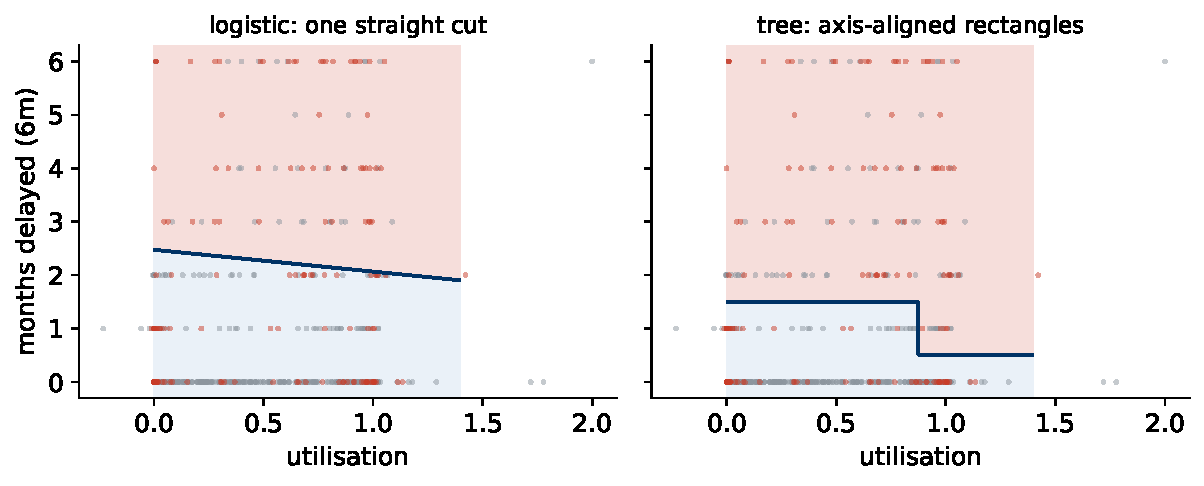
\includegraphics[width=0.85\textwidth]{figures/fig_boundaries.pdf}
  \end{center}
  \begin{itemize}\small
    \item Same two features, same data: logistic draws \alert{one straight
          cut}; the tree tiles the space with \alert{axis-aligned rectangles}.
    \item More rectangles = more flexibility = a longer walk down the
          U-curve. The leash question is coming.
  \end{itemize}
\end{frame}

% ---------------------------------------------------------------
\begin{frame}{Anatomy of a fitted tree (ours, depth 2)}
  \begin{center}
    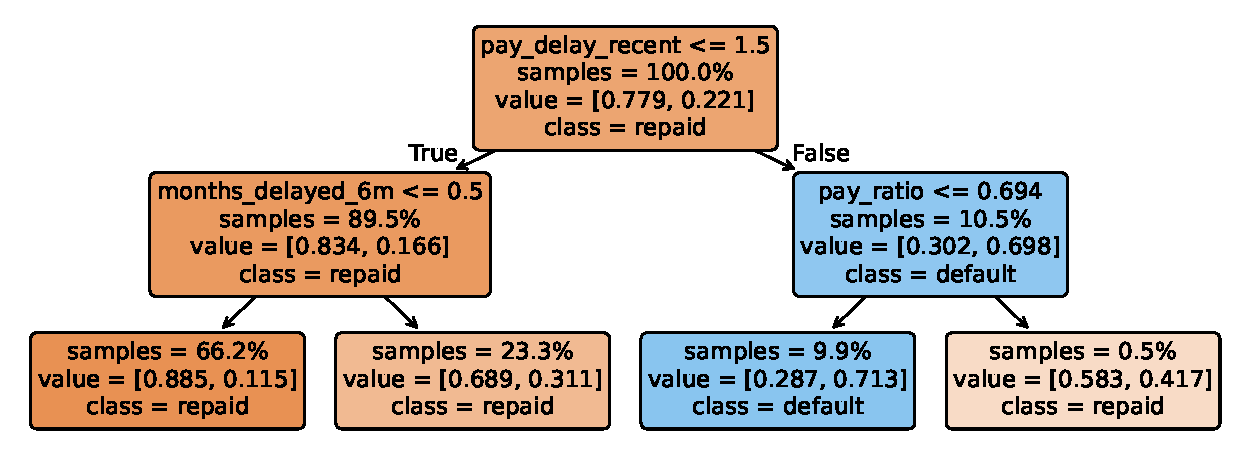
\includegraphics[width=0.85\textwidth]{figures/fig_tree_example.pdf}
  \end{center}
  \begin{itemize}\small
    \item Predicting = walking one path from root to leaf; the leaf's class
          mix is the probability estimate. Reading a path aloud gives an
          \alert{explanation for free}.
    \item Look at the root: the tree opens with
          \texttt{pay\_delay\_recent} at the \alert{two-months-behind
          cliff} - agreeing with the logistic coefficients that payment
          history is where the signal lives. Two very different algorithms,
          same verdict.
  \end{itemize}
\end{frame}

% ---------------------------------------------------------------
\begin{frame}{How a split is chosen}
  At every node, try every feature and every cut-point; keep the split that
  makes the children \alert{purest}:
  \[
    \text{Gini}(node) = 1 - p_0^2 - p_1^2
    \qquad
    \Delta = \text{Gini}_{\text{parent}}
    - \tfrac{n_L}{n}\,\text{Gini}_L - \tfrac{n_R}{n}\,\text{Gini}_R
  \]
  \begin{itemize}\small
    \item $p_k$ = class shares in the node. Pure leaf: Gini $= 0$;
          50/50 node: Gini $= 0.5$. (Entropy,
          $-\sum_k p_k \log_2 p_k$, is the same idea with logs -
          rankings of splits rarely differ.)
    \item Growth is \alert{greedy}: best split \emph{now}, no lookahead -
          fast, and not guaranteed optimal.
    \item Repeat recursively until a stopping rule (the leash) says stop.
  \end{itemize}
\end{frame}

% ---------------------------------------------------------------
\begin{frame}{Gini by hand (exam-friendly)}
  Parent node: 1{,}000 customers, 30\% default.
  \[
    \text{Gini}_{\text{parent}} = 1 - 0.7^2 - 0.3^2 = 0.42
  \]
  Candidate split on \texttt{utilisation} $> 0.6$:
  \begin{center}\small
  \begin{tabular}{@{}lccc@{}}
    \toprule
    Child & $n$ & default rate & Gini \\
    \midrule
    left (low util.) & 600 & 10\% & $1 - 0.9^2 - 0.1^2 = 0.18$ \\
    right (high util.) & 400 & 60\% & $1 - 0.4^2 - 0.6^2 = 0.48$ \\
    \bottomrule
  \end{tabular}
  \end{center}
  \[
    \text{weighted} = 0.6 \times 0.18 + 0.4 \times 0.48 = 0.30
    \qquad
    \Delta = 0.42 - 0.30 = \alert{0.12}
  \]
  \begin{center}\small
    The algorithm computes this $\Delta$ for every feature $\times$ every
    cut-point - and picks the maximum. That's the whole magic.
  \end{center}
\end{frame}

% ---------------------------------------------------------------
\begin{frame}{Where is the tree's leash?}
  \begin{center}
    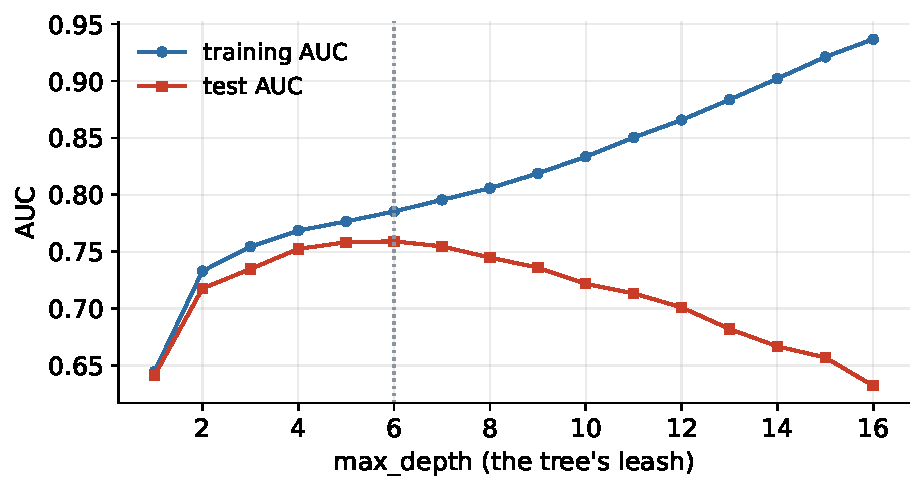
\includegraphics[width=0.6\textwidth]{figures/fig_tree_depth.pdf}
  \end{center}
  \begin{itemize}\small
    \item Unleashed, a tree memorises: training AUC $\to 1$ while test AUC
          \alert{falls} - the U-curve, tree edition. Best here: depth
          $\approx$6 (30{,}000 rows feed a deeper tree than Block 1's
          4{,}000 ever could); beyond that, memorisation.
    \item Leashes: \texttt{max\_depth}, \texttt{min\_samples\_leaf} (no
          leaf smaller than\ldots), pruning. Same logic as $\alpha$ last week.
  \end{itemize}
\end{frame}

% ---------------------------------------------------------------
\begin{frame}{A single tree's pathologies}
  \begin{itemize}
    \item \textbf{High variance.} Nudge the training data and the first
          split flips - and everything below it changes. One tree is
          a \alert{nervous} model.
    \item \textbf{Steps, not slopes.} Within a leaf the prediction is
          constant: risk that plainly grows with utilisation becomes a
          staircase.
    \item \textbf{Extrapolation, worse edition.} Beyond the training range a
          tree predicts the \emph{edge leaf's} value - flat forever.
          (Block 2's warning, now with a flatline.)
  \end{itemize}
  \vspace{0.5em}
  \begin{center}
    Fix the staircase with depth; fix the nerves with \alert{many trees} -
    next section.
  \end{center}
\end{frame}

% ---------------------------------------------------------------
\begin{frame}{Regression trees exist too}
  \begin{itemize}
    \item Same machinery, numeric target: leaves predict the \alert{mean} of
          their training rows; splits minimise variance (MSE) instead of Gini.
    \item Same pathologies (staircase, variance) - and the same leash.
    \item Why care today: gradient boosting fits \alert{regression trees to
          errors} even for classification - you need this piece to
          understand GBDT in ten minutes.
  \end{itemize}
  \vspace{0.5em}
  \begin{center}\small
    Credit uses them directly, too: LGD and exposure models are regression
    problems (Block 2's map).
  \end{center}
\end{frame}

% ---------------------------------------------------------------
\begin{frame}{What trees \emph{don't} need}
  \begin{itemize}
    \item \textbf{No scaling.} Splits compare against cut-points; units are
          irrelevant. (The scaler stays in the pipeline for the logistic
          baseline only.)
    \item \textbf{No monotone transforms.} $\log(\text{income})$ and income
          give identical trees - splits are order-based.
    \item \textbf{Ordinal encodings suffice.} Trees can cut an ordered code
          anywhere; the dummy trap is a linear-model disease.
    \item \textbf{Missing values}: plain sklearn trees still want
          imputation, but \texttt{HistGradientBoosting} handles NaN
          \alert{natively} - it learns which side missing values should go.
          Block 1's structural NaN can stay a NaN.
  \end{itemize}
  \vspace{0.4em}
  \begin{center}\small
    Less preprocessing $\ne$ no thinking: the time-travel test and the
    missingness taxonomy still apply in full.
  \end{center}
\end{frame}

% ---------------------------------------------------------------
\begin{frame}{Tree vs logistic, side by side}
  \small
  \begin{center}
  \begin{tabular}{@{}lll@{}}
    \toprule
     & Logistic regression & Decision tree \\
    \midrule
    Boundary & one straight cut & axis-aligned rectangles \\
    Interactions & engineered by hand & found automatically \\
    Scaling / transforms & required (penalties) & irrelevant \\
    Missing values & impute + indicator & (Hist)GBDT: native \\
    Output & calibrated-ish probabilities & leaf frequencies, chunky \\
    Stability & high & \alert{low - nervous} \\
    Explanation & coefficients, odds ratios & the path itself \\
    \bottomrule
  \end{tabular}
  \end{center}
  \vspace{0.5em}
  \begin{center}
    Neither dominates. The interesting question is what happens when trees
    \alert{stop working alone}.
  \end{center}
\end{frame}

% ============================================================
% SECTION: SVM INTERLUDE
% ============================================================
\section{SVM}

% ---------------------------------------------------------------
\begin{frame}{Interlude: the widest street (support vector machines)}
  \begin{columns}[T]
    \begin{column}{0.5\textwidth}
      \begin{center}
        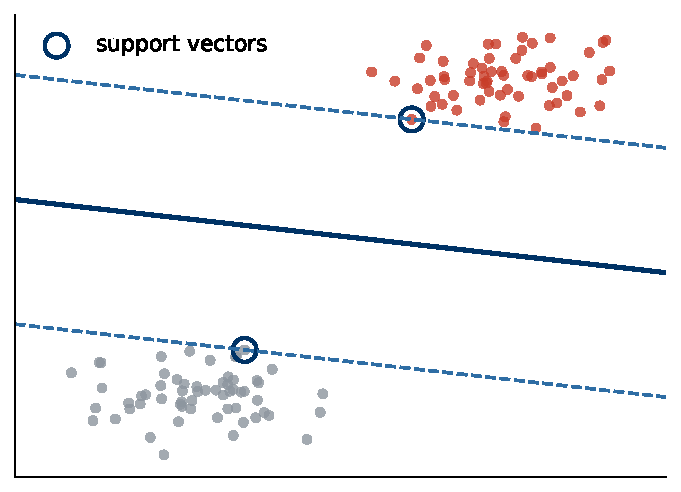
\includegraphics[width=0.94\linewidth]{figures/fig_svm_margin.pdf}
      \end{center}
    \end{column}
    \begin{column}{0.48\textwidth}
      \vspace{0.3em}
      \small
      Among all separating lines, pick the one with the \alert{widest
      margin}:
      \[
        \min_{w, b}\; \tfrac{1}{2}\lVert w \rVert^2
        \;\;\text{s.t.}\;\; y_i (w \cdot x_i + b) \geq 1
      \]
      (margin width $= 2/\lVert w \rVert$; soft version adds
      $C \sum_i \xi_i$ for violations)
      \begin{itemize}\small
        \item The line is held up only by the \alert{support vectors} -
              the circled border cases; everyone else could vanish.
        \item Wide street $=$ built-in caution about new customers near
              the boundary.
      \end{itemize}
    \end{column}
  \end{columns}
\end{frame}

% ---------------------------------------------------------------
\begin{frame}{The kernel trick: bending without leaving linear algebra}
  \begin{center}
    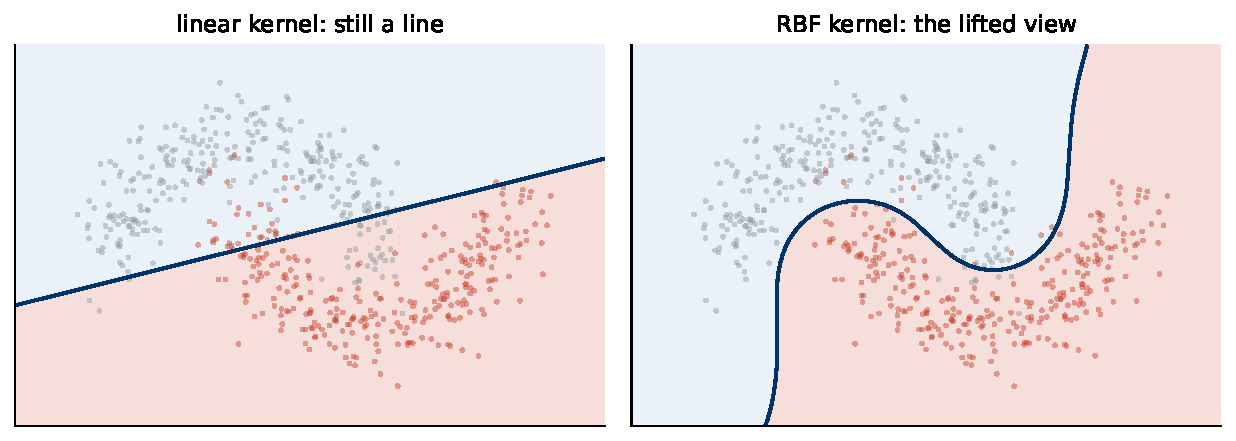
\includegraphics[width=0.8\textwidth]{figures/fig_svm_kernel.pdf}
  \end{center}
  \begin{itemize}\small
    \item Idea: map points into a higher-dimensional space where a
          \emph{line} suffices - computed implicitly through a
          \alert{kernel} $K(x, x') = \varphi(x) \cdot \varphi(x')$,
          never building $\varphi$ at all.
    \item The workhorse RBF kernel,
          $K(x, x') = \exp(-\gamma \lVert x - x' \rVert^2)$: similarity
          decays with distance - and $\gamma$ is (say it with me)
          \alert{the leash}.
    \item Third route to nonlinearity this course: engineered features
          (B2), tree splits (today), kernels.
  \end{itemize}
\end{frame}

% ---------------------------------------------------------------
\begin{frame}{SVM in one loss curve - and in practice}
  \begin{center}
    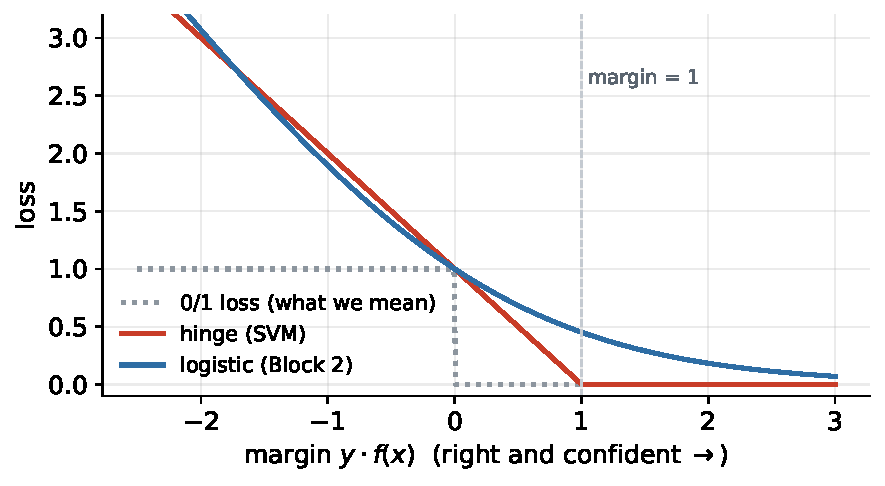
\includegraphics[width=0.48\textwidth]{figures/fig_losses.pdf}
  \end{center}
  \begin{itemize}\small
    \item Hinge loss $\max(0,\, 1 - y f(x))$: zero once you are right
          \emph{with margin} - vs Block 2's logistic loss, which never
          fully forgives. Same recipe as everything else:
          loss $+$ leash, minimised.
    \item Practice: scale first (distances again); no native
          probabilities (calibrate before pricing); training scales
          poorly past $\sim$10$^5$ rows - one reason GBDT took its
          tabular crown.
    \item On our PD task (trained on a 6{,}000-row subsample - the
          $n^2$ cost is real): test AUC \alert{0.715}, behind the logistic
          baseline (0.731). Kernels buy bend, but not as cheaply as trees
          buy the delay cliff - next section.
  \end{itemize}
\end{frame}

% ============================================================
% SECTION: ENSEMBLES
% ============================================================
\section{Ensembles}

% ---------------------------------------------------------------
\begin{frame}{One tree is nervous - so ask a crowd}
  \begin{itemize}
    \item Average many over-flexible, \emph{differently-wrong} models and
          the individual errors partially \alert{cancel}: variance drops,
          bias stays.
    \item The catch: trees grown on the same data make the \emph{same}
          mistakes - averaging clones buys nothing.
    \item Ensembling = manufacturing \alert{disagreement} between good
          models, then averaging it away.
  \end{itemize}
  \vspace{0.6em}
  \begin{block}{Two ways to manufacture disagreement}
    \textbf{Bagging}: give each tree different \emph{data}.
    \quad
    \textbf{Boosting}: give each tree a different \emph{job}.
  \end{block}
\end{frame}

% ---------------------------------------------------------------
\begin{frame}{Bagging: bootstrap + aggregate}
  \begin{itemize}
    \item \textbf{Bootstrap}: sample $n$ rows \emph{with replacement} -
          each tree trains on its own resampled portfolio ($\sim$63\% unique
          rows).
    \item Grow each tree deep (low bias, high variance), then
          \textbf{aggregate}: average the probabilities.
    \item Free lunch included: each tree never saw $\sim$37\% of rows -
          its \alert{out-of-bag} (OOB) rows give validation-like feedback
          without a split.
  \end{itemize}
  \vspace{0.6em}
  \begin{center}
    Variance falls like an average of noisy measurements - as long as the
    trees genuinely \alert{disagree}.
  \end{center}
\end{frame}

% ---------------------------------------------------------------
\begin{frame}{Random forest = bagging + a feature lottery}
  \begin{itemize}
    \item Problem: with one dominant feature (say, utilisation), every
          bootstrap tree still opens with the \emph{same split} -
          correlated trees, weak averaging.
    \item Fix: at every node, allow only a \alert{random subset of features}
          (\texttt{max\_features}) to compete.
    \item Forced variety $\Rightarrow$ decorrelated trees $\Rightarrow$
          averaging actually works. That one trick is the ``random'' in
          random forest.
  \end{itemize}
  \vspace{0.6em}
  \begin{center}\small
    Practical defaults: hundreds of deep trees,
    \texttt{max\_features} $\approx \sqrt{p}$,
    \texttt{min\_samples\_leaf} as the leash.
  \end{center}
\end{frame}

% ---------------------------------------------------------------
\begin{frame}{How many trees?}
  \begin{center}
    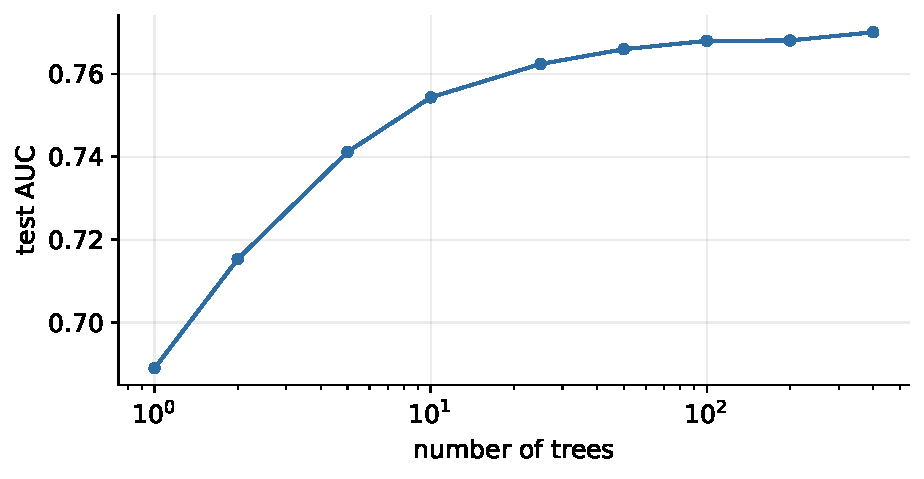
\includegraphics[width=0.68\textwidth]{figures/fig_rf_ntrees.pdf}
  \end{center}
  \begin{itemize}\small
    \item Test AUC climbs, then \alert{plateaus} - more trees never
          overfit; they only cost compute.
    \item So \texttt{n\_estimators} is not really a tuning knob: set it
          ``large enough'' and tune the \emph{tree-level} leashes instead.
  \end{itemize}
\end{frame}

% ---------------------------------------------------------------
\begin{frame}{Boosting: a different philosophy}
  \begin{itemize}
    \item Bagging builds trees \emph{in parallel} and averages equals.
          Boosting builds them \alert{in sequence}: each new tree fits the
          \emph{errors} of the ensemble so far.
    \item ``Errors'' precisely: the \alert{gradient} of the loss (log-loss
          for us) - hence \emph{gradient} boosting. Each round is a small
          regression tree on those gradients (told you they'd matter).
    \item Predictions accumulate: $F_{m}(x) = F_{m-1}(x) + \eta \cdot
          \text{tree}_m(x)$, with learning rate $\eta$ keeping steps humble.
  \end{itemize}
  \vspace{0.5em}
  \begin{center}
    Bagging attacks \alert{variance}; boosting attacks \alert{bias} -
    and can therefore overfit, so its leash matters more.
  \end{center}
\end{frame}

% ---------------------------------------------------------------
\begin{frame}{GBDT's knobs - and a cautionary tale}
  \begin{itemize}\small
    \item \textbf{Learning rate $\times$ rounds}: small steps, more of them
          - the classic robust recipe.
    \item \textbf{Shallow trees} (depth 2--4 / few leaves): each round adds
          a weak, humble learner.
    \item \textbf{Early stopping}: watch a validation slice, stop when it
          stops improving - GBDT's leash.
  \end{itemize}
  \vspace{0.4em}
  \begin{alertblock}{Leashes are sized to the data}
    On this 21{,}000-row training set, sklearn's default GBDT already
    scores \textbf{0.774} - defaults are tuned for data this size. The
    same defaults on Block 1's little synthetic portfolio scored 0.651
    against 0.714 tuned: small data needs short leashes. Check, never
    assume - in either direction.
  \end{alertblock}
  \vspace{0.3em}
  \begin{center}\small
    Industry names for the same idea: XGBoost, LightGBM, CatBoost.
  \end{center}
\end{frame}

% ---------------------------------------------------------------
\begin{frame}{RF vs GBDT}
  \small
  \begin{center}
  \begin{tabular}{@{}lll@{}}
    \toprule
     & Random forest & GBDT \\
    \midrule
    Trees built & in parallel, independent & in sequence, corrective \\
    Attacks & variance & bias (then overfits) \\
    Tree size & deep & shallow \\
    Key leash & leaf size, feature lottery & rate, rounds, early stop \\
    Tuning effort & low - hard to ruin & moderate - easy to ruin \\
    Typical tabular result & strong & \alert{state of the art} \\
    \bottomrule
  \end{tabular}
  \end{center}
  \vspace{0.5em}
  \begin{center}\small
    Rule of thumb: RF as the robust first ensemble; GBDT when you are ready
    to tune - and to validate properly.
  \end{center}
\end{frame}

% ---------------------------------------------------------------
\begin{frame}{The tournament on our portfolio}
  \begin{center}
    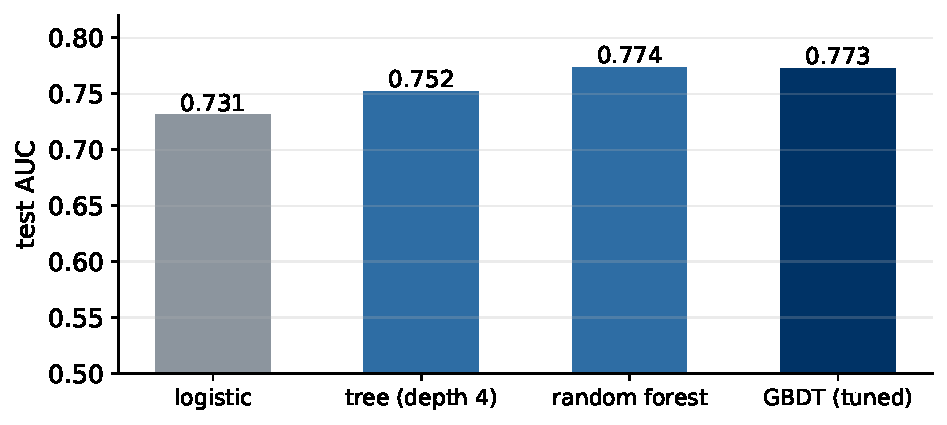
\includegraphics[width=0.72\textwidth]{figures/fig_model_comparison.pdf}
  \end{center}
  \begin{itemize}\small
    \item \alert{Every rung of the ladder pays}: logistic 0.731 $\to$
          single tree 0.752 $\to$ forest 0.774 / tuned GBDT 0.773.
    \item On real behavioural data, complexity \alert{earns its keep} -
          about +4 AUC points from baseline to ensemble. Is that gap real?
          The CV section will certify it.
  \end{itemize}
\end{frame}

% ---------------------------------------------------------------
\begin{frame}{Why complexity wins \emph{here} - and didn't in Block 1's world}
  \begin{itemize}
    \item The real portfolio is full of what linear models must be
          \alert{hand-fed}: the repayment-status \alert{cliff} (one missed
          month is news; the second is a siren), saturating utilisation,
          delay $\times$ limit interactions. Trees carve these natively.
    \item Block 1's synthetic world was additive in log-odds by
          construction - logistic regression's home turf, and complexity
          politely declined there. Same course, both outcomes, both honest.
    \item The meta-lesson outlives both datasets.
  \end{itemize}
  \vspace{0.5em}
  \begin{block}{You cannot know in advance}
    Which family wins is an \emph{empirical} question, decided per dataset,
    against a baseline, on honest numbers. Never by fashion.
  \end{block}
\end{frame}

% ---------------------------------------------------------------
\begin{frame}{Tuning without tears}
  \begin{itemize}
    \item \textbf{Start from defaults}, change one leash at a time; keep a
          log (Block 1's evidence discipline).
    \item \textbf{Random search beats grid search} for the same budget -
          important knobs get more distinct values.
    \item \textbf{Tune on cross-validation, confirm on test} - the
          three-samples contract from Block 2, now load-bearing.
    \item \textbf{Stop early}: tuning yields little once the leash is
          roughly right; feature work usually pays more (Block 1, always
          Block 1).
  \end{itemize}
  \vspace{0.5em}
  \begin{center}\small
    sklearn: \texttt{RandomizedSearchCV} - CV built in, pipeline-friendly.
  \end{center}
\end{frame}

% ============================================================
% SECTION: EVALUATION
% ============================================================
\section{Evaluation}

% ---------------------------------------------------------------
\begin{frame}{Why one split can lie}
  \begin{itemize}
    \item Our test set is 9{,}000 customers - \alert{one draw} from the
          space of possible test sets. A lucky draw flatters; an unlucky one
          slanders.
    \item At this size the noise is smaller, but differences of a few tenths
          of a point of AUC can still be \emph{sampling noise}, not model
          quality - and most real projects have far fewer rows.
    \item We compared four models on that single draw last section -
          how much should we trust the ranking?
  \end{itemize}
  \vspace{0.6em}
  \begin{center}
    We need a \alert{distribution} of scores, not a point.
    Enter cross-validation.
  \end{center}
\end{frame}

% ---------------------------------------------------------------
\begin{frame}{$k$-fold cross-validation}
  \begin{center}
  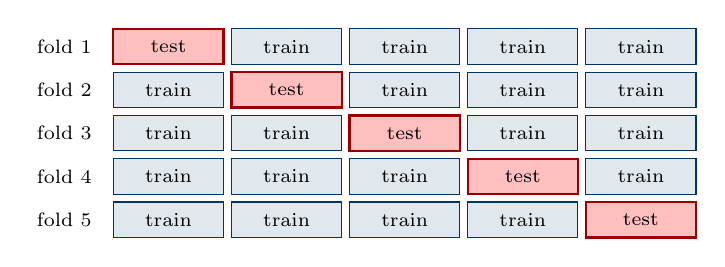
\begin{tikzpicture}[font=\scriptsize]
    \foreach \r in {0,...,4} {
      \foreach \c in {0,...,4} {
        \ifnum\r=\c
          \fill[red!25] (\c*1.5, -\r*0.55) rectangle ++(1.4, 0.45);
          \draw[red!60!black, thick] (\c*1.5, -\r*0.55) rectangle ++(1.4, 0.45);
          \node at (\c*1.5+0.7, -\r*0.55+0.225) {test};
        \else
          \fill[sghblue!12] (\c*1.5, -\r*0.55) rectangle ++(1.4, 0.45);
          \draw[sghblue] (\c*1.5, -\r*0.55) rectangle ++(1.4, 0.45);
          \node at (\c*1.5+0.7, -\r*0.55+0.225) {train};
        \fi
      }
      \node[anchor=east] at (-0.15, -\r*0.55+0.225) {fold \the\numexpr\r+1\relax};
    }
  \end{tikzpicture}
  \end{center}
  \vspace{0.5em}
  \begin{itemize}\small
    \item Split the \emph{training} data into $k$ folds; train on $k-1$,
          score on the held-out fold; rotate. Every row gets scored
          \alert{exactly once} by a model that never saw it.
    \item Output: $k$ scores $\to$ \alert{mean $\pm$ spread}. ($k = 5$ or 10;
          stratified for classification.)
  \end{itemize}
\end{frame}

% ---------------------------------------------------------------
\begin{frame}{CV on our portfolio}
  \begin{center}
    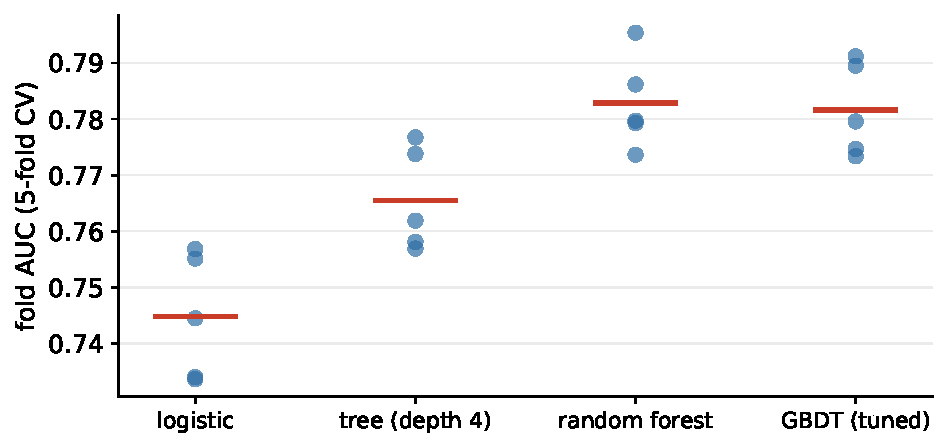
\includegraphics[width=0.66\textwidth]{figures/fig_cv_spread.pdf}
  \end{center}
  \begin{itemize}\small
    \item Logistic $0.745 \pm 0.010$, tree $0.766 \pm 0.008$, forest
          $0.783 \pm 0.007$: at 21{,}000 training rows the spreads are
          \alert{tight} - and the tree-vs-logistic gap ($\sim$0.02) clears
          its spread several times over. \alert{Certified, not lucky.}
    \item Report mean $\pm$ sd, always. A model ``winning'' by less than the
          spread hasn't won anything yet - and now you can tell.
  \end{itemize}
\end{frame}

% ---------------------------------------------------------------
\begin{frame}{CV hygiene}
  \begin{enumerate}
    \item \textbf{Stratify} the folds - each fold keeps the 22\% default
          rate.
    \item \textbf{The pipeline goes \emph{inside}} - scaler, imputer,
          encoder refit on each fold's training part.
          Fitting transforms once on all data leaks across every fold
          boundary. \alert{This is why pipelines exist.}
    \item \textbf{CV chooses, the test set confirms} - hyperparameters and
          model family are picked on CV; the untouched test set delivers one
          final number.
    \item \textbf{Never} cross-validate on data that includes your test set.
  \end{enumerate}
  \vspace{0.4em}
  \begin{center}\small
    $k = 5$: cheaper, noisier. $k = 10$: slower, tighter. Repeated CV when
    the decision is close.
  \end{center}
\end{frame}

% ---------------------------------------------------------------
\begin{frame}{Time makes splits harder}
  \begin{itemize}
    \item Credit portfolios \alert{drift}: products change, policies change
          (selection bias, Block 1!), the economy cycles.
    \item Random CV mixes 2023 and 2025 customers in both directions -
          the model ``sees the future'' and scores optimistically.
    \item The credit standard: \textbf{out-of-time validation} - train on
          the past, test on a later window; CV \emph{within} the training
          period for tuning.
    \item Our synthetic portfolio has no dates - your project data or your
          first job will. Ask ``\alert{does time matter here?}'' before
          every split.
  \end{itemize}
\end{frame}

% ---------------------------------------------------------------
\begin{frame}{Beyond one threshold: judge the ranking}
  \begin{itemize}
    \item Last week's precision and recall judged the model \emph{at one
          threshold} - one confusion matrix out of a continuum.
    \item But the threshold belongs to the business and may move. What we
          should judge first is the model's \alert{ordering} of customers by
          risk.
    \item Idea: sweep the threshold from 1 to 0, trace what happens to the
          error rates - every threshold becomes one point of a curve.
  \end{itemize}
  \vspace{0.6em}
  \begin{center}
    That curve is the \alert{ROC}; its area is the ranking's quality.
  \end{center}
\end{frame}

% ---------------------------------------------------------------
\begin{frame}{The ROC curve}
  \begin{columns}[T]
    \begin{column}{0.52\textwidth}
      \begin{center}
        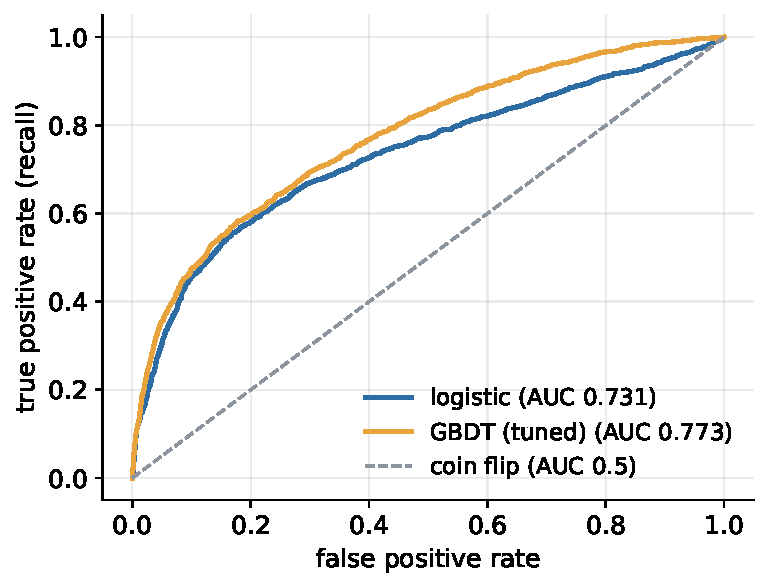
\includegraphics[width=\linewidth]{figures/fig_roc.pdf}
      \end{center}
    \end{column}
    \begin{column}{0.46\textwidth}
      \vspace{0.8em}
      \begin{itemize}\small
        \item $x$: false positive rate (good customers flagged);
              $y$: true positive rate (defaulters caught).
        \item Each point = one threshold; the diagonal = coin flip.
        \item Choosing an \alert{operating point} on this curve \emph{is}
              choosing a threshold - the business conversation, drawn.
      \end{itemize}
    \end{column}
  \end{columns}
\end{frame}

% ---------------------------------------------------------------
\begin{frame}{AUC: one number for the ranking}
  \begin{block}{The probabilistic meaning (memorise this one)}
    AUC $=$ the probability that a randomly chosen \emph{defaulter} is
    scored riskier than a randomly chosen \emph{good customer}.
  \end{block}
  \vspace{0.4em}
  \begin{itemize}\small
    \item Anchors: $0.5$ = dice; $1.0$ = crystal ball. Ours: logistic
          $0.731$, tuned GBDT $0.773$.
    \item Threshold-free and insensitive to class imbalance - judges the
          \emph{ranking}, nothing else.
    \item What it does \alert{not} tell you: whether probabilities are
          honest (calibration) or what a decision costs (thresholding).
          Three questions, three tools.
  \end{itemize}
\end{frame}

% ---------------------------------------------------------------
\begin{frame}{The credit dialect: Gini and KS}
  \begin{itemize}
    \item Credit scoring rarely says ``AUC''. It says \alert{Gini}:
    \[
      \text{Gini} = 2 \cdot \text{AUC} - 1
      \qquad \text{(ours: logistic } 0.46\text{, GBDT } 2 \times 0.773 - 1 \approx \alert{0.55}\text{)}
    \]
    \item Same information, rescaled: dice $= 0$, crystal ball $= 1$.
          A retail PD model with Gini 0.4--0.6 is normal furniture.
    \item You will also meet \textbf{KS}: the maximum gap between the score
          distributions of goods and bads - one more ranking statistic,
          same family.
    \item Interview survival tip: when a risk manager says Gini, they mean
          this - \alert{not} the Gini impurity from the tree section.
          Same Corrado Gini, different formula.
  \end{itemize}
\end{frame}

% ---------------------------------------------------------------
\begin{frame}{Precision--recall: when positives are rare}
  \begin{columns}[T]
    \begin{column}{0.52\textwidth}
      \begin{center}
        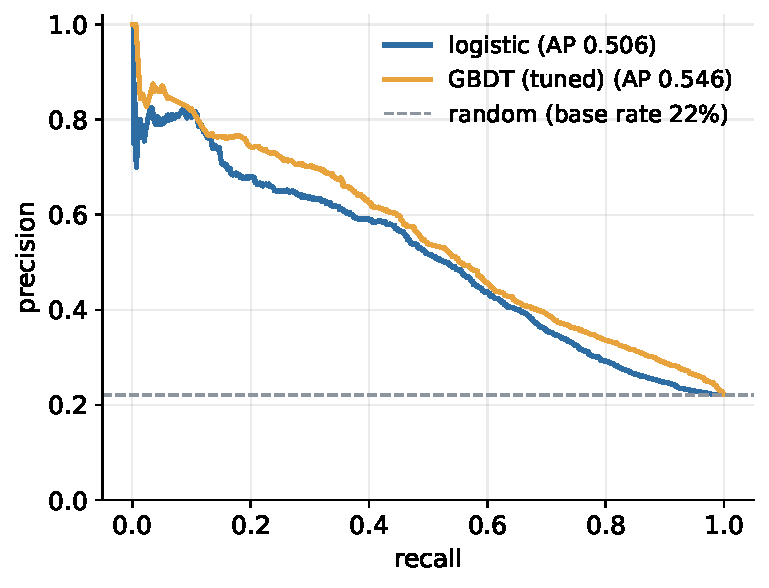
\includegraphics[width=\linewidth]{figures/fig_pr.pdf}
      \end{center}
    \end{column}
    \begin{column}{0.46\textwidth}
      \vspace{0.8em}
      \begin{itemize}\small
        \item Random guessing floors at the \alert{base rate} (here 22\%) -
              PR curves punish false alarms among rare positives.
        \item At 1--5\% default rates (or fraud's 0.1\%), ROC can look
              flattering while precision is dismal - check \alert{both}.
        \item One number: average precision (AP).
      \end{itemize}
    \end{column}
  \end{columns}
\end{frame}

% ---------------------------------------------------------------
\begin{frame}{Calibration: is a predicted 0.3 really a 0.3?}
  \begin{columns}[T]
    \begin{column}{0.52\textwidth}
      \begin{center}
        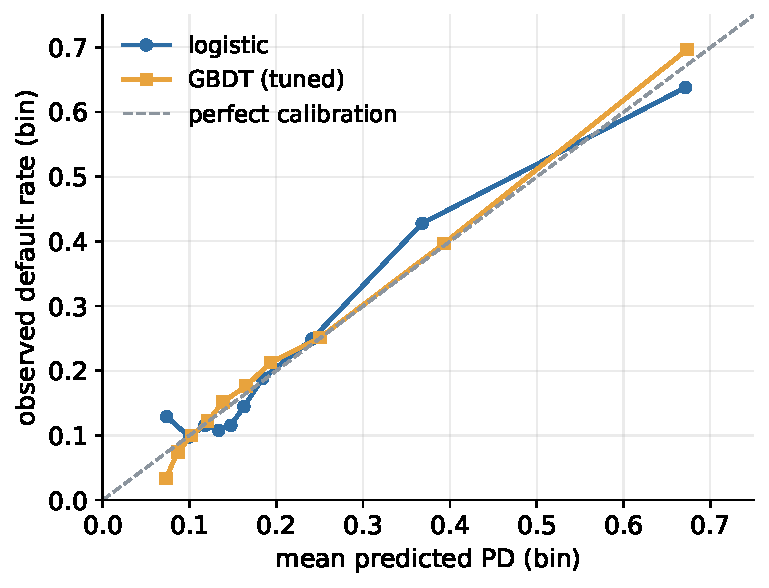
\includegraphics[width=\linewidth]{figures/fig_calibration.pdf}
      \end{center}
    \end{column}
    \begin{column}{0.46\textwidth}
      \vspace{0.6em}
      \begin{itemize}\small
        \item Bin customers by predicted PD; compare with the bin's
              \emph{observed} default rate. Diagonal = honest.
        \item Ranking pays for \alert{approval order}; calibration pays for
              \alert{pricing and provisions} - interest rates are set on
              the probability itself.
        \item Repairs exist: Platt scaling, isotonic regression
              (\texttt{CalibratedClassifierCV}). And recall Block 2:
              \texttt{class\_weight} \alert{breaks} calibration by design.
      \end{itemize}
    \end{column}
  \end{columns}
\end{frame}

% ---------------------------------------------------------------
\begin{frame}{From metrics to money: expected cost}
  \vspace{-0.4em}
  {\small
  \[
    \mathrm{E}[\text{cost}](t) \;=\;
    \frac{C_{FN} \cdot FN(t) \;+\; C_{FP} \cdot FP(t)}{n}
    \qquad t^{*} = \arg\min_t \mathrm{E}[\text{cost}](t)
  \]}
  \begin{center}
    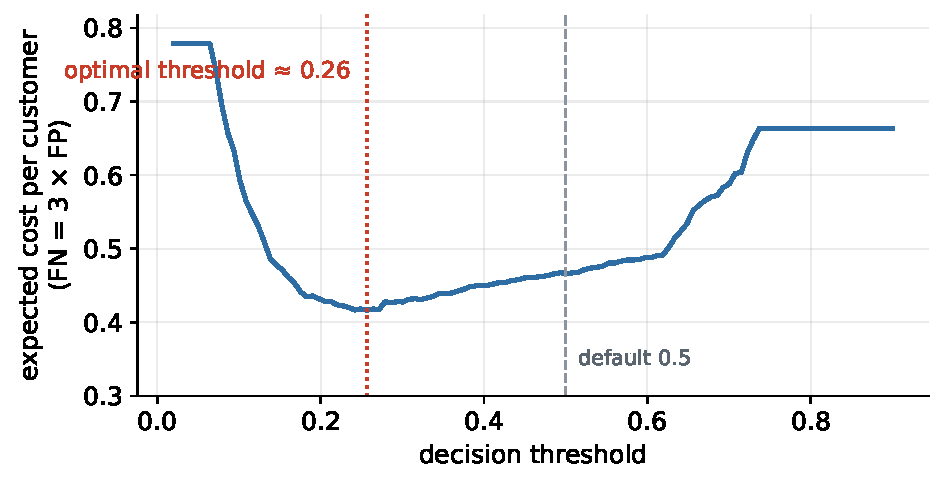
\includegraphics[width=0.54\textwidth]{figures/fig_expected_cost.pdf}
  \end{center}
  \begin{itemize}\small
    \item Price the cells (here $C_{FN} = 3 \times C_{FP}$; real low-default
          books push $10$--$50\times$), sweep the threshold, minimise.
    \item Optimum $\approx \alert{0.26}$, not 0.5 - and the move cuts
          expected cost by \alert{$\sim$11\%}. Same model, better decision.
          Block 2's cliffhanger: resolved.
  \end{itemize}
\end{frame}

% ---------------------------------------------------------------
\begin{frame}{The PD evaluation stack}
  \small
  \begin{center}
  \begin{tabular}{@{}clll@{}}
    \toprule
    \# & Question & Tool & Frequency \\
    \midrule
    1 & Does it rank risk? & AUC / Gini, CV mean $\pm$ sd & every model \\
    2 & Are probabilities honest? & calibration curve, recalibrate & before pricing \\
    3 & Where do we cut? & expected cost vs threshold & with the business \\
    4 & Does it stay good? & out-of-time tests, monitoring & forever \\
    \bottomrule
  \end{tabular}
  \end{center}
  \vspace{0.6em}
  \begin{center}
    In that order. A perfectly calibrated model that ranks badly prices
    garbage accurately; a great ranker with dishonest probabilities
    misprices everything.
  \end{center}
\end{frame}

% ---------------------------------------------------------------
\begin{frame}{Metric cheat sheet}
  \footnotesize
  \begin{center}
  \begin{tabular}{@{}llll@{}}
    \toprule
    Metric & Question & Threshold-bound? & Classic trap \\
    \midrule
    Accuracy & share correct & yes & lies under imbalance \\
    Precision & flagged $\to$ right? & yes & ignores missed positives \\
    Recall (TPR) & positives caught? & yes & 100\% by flagging everyone \\
    F1 & precision+recall blend & yes & blind to costs and TNs \\
    AUC / Gini & ranking quality & no & says nothing about calibration \\
    Average precision & ranking, rare positives & no & less intuitive to explain \\
    Calibration error & honest probabilities? & no & great ranking can hide it \\
    Expected cost & money at the cut-off & yes & needs costs you must ask for \\
    \bottomrule
  \end{tabular}
  \end{center}
  \vspace{0.4em}
  \begin{center}\small
    One rule survives every situation: \alert{never a single metric, never
    on training data} - now with a toolbox behind it.
  \end{center}
\end{frame}

% ============================================================
% SECTION: LEAKAGE
% ============================================================
\section{Leakage}

% ---------------------------------------------------------------
\begin{frame}{The suspect has been in the room since Block 1}
  \begin{itemize}
    \item \texttt{collections\_contact} - ``did collections call this
          customer?'' - shipped with the portfolio on day one, flagged
          \alert{do not use}.
    \item Time-travel test: collections calls happen mostly \emph{after}
          default. At application time this value \alert{does not exist}.
    \item Today we do what you should never do in production -
          on purpose, with instruments attached.
  \end{itemize}
  \vspace{0.6em}
  \begin{center}
    Hypothesis: the model will look \alert{magnificent}.
  \end{center}
\end{frame}

% ---------------------------------------------------------------
\begin{frame}{The detonation}
  \begin{center}
    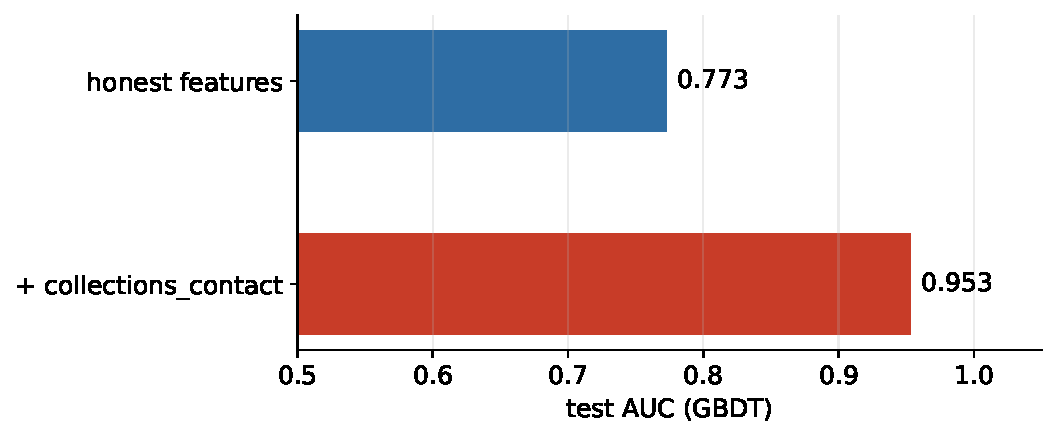
\includegraphics[width=0.8\textwidth]{figures/fig_leakage.pdf}
  \end{center}
  \begin{itemize}\small
    \item One added column: AUC $0.773 \to \alert{0.953}$. The best model
          this course will ever produce - and \alert{completely worthless}:
          in production the feature is unknowable at decision time.
    \item Nothing crashed. No warning fired. The only alarms were
          \emph{yours}: the time-travel test, and ``too good to be true''.
  \end{itemize}
\end{frame}

% ---------------------------------------------------------------
\begin{frame}{Why leakage is so seductive}
  \begin{itemize}
    \item The leaky feature looks like your \alert{best feature} -
          importance rankings crown it instantly.
    \item Every honest check passes: CV loves it, the test set loves it
          - because the leak sits on \emph{both} sides of every split.
    \item The only failing dataset is the one you don't have yet:
          \alert{production}.
    \item Which is why leakage is caught by \emph{reasoning about features},
          not by metrics: metrics are its accomplices.
  \end{itemize}
\end{frame}

% ---------------------------------------------------------------
\begin{frame}{A leakage bestiary}
  \small
  \begin{center}
  \begin{tabular}{@{}lp{6.4cm}@{}}
    \toprule
    Species & Example \\
    \midrule
    Post-outcome field & \texttt{collections\_contact}, \texttt{account\_closed\_reason} \\
    Target twin & \texttt{months\_overdue} predicting default \\
    Transform leak & scaler / imputer / encoder fitted on all data \\
    Duplicate leak & same customer lands in train \emph{and} test \\
    Group leak & multiple loans of one person split across sides \\
    Time-travel join & feature table joined with post-decision snapshot \\
    \bottomrule
  \end{tabular}
  \end{center}
  \vspace{0.4em}
  \begin{center}\small
    The last three are the sneaky ones: no single column looks guilty -
    the \emph{procedure} leaks.
  \end{center}
\end{frame}

% ---------------------------------------------------------------
\begin{frame}{The smell test \& the checklist}
  \textbf{Smells (any one $\Rightarrow$ stop and audit)}
  \begin{itemize}\small
    \item AUC far above the domain's normal range (retail PD: Gini 0.4--0.6)
    \item one feature dominating importance
    \item test score $\gg$ CV score, or CV suspiciously tight
  \end{itemize}
  \vspace{0.4em}
  \textbf{Checklist (before believing any good result)}
  \begin{itemize}\small
    \item every feature has an answer to ``\alert{when is this value
          known?}'' - written down
    \item all transforms live inside the pipeline; keys checked for
          duplicates; groups split together
    \item time in the data $\Rightarrow$ out-of-time test exists
  \end{itemize}
\end{frame}

% ============================================================
% SECTION: EXPLANATIONS
% ============================================================
\section{Explanations}

% ---------------------------------------------------------------
\begin{frame}{Which features matter? Two answers}
  \begin{center}
    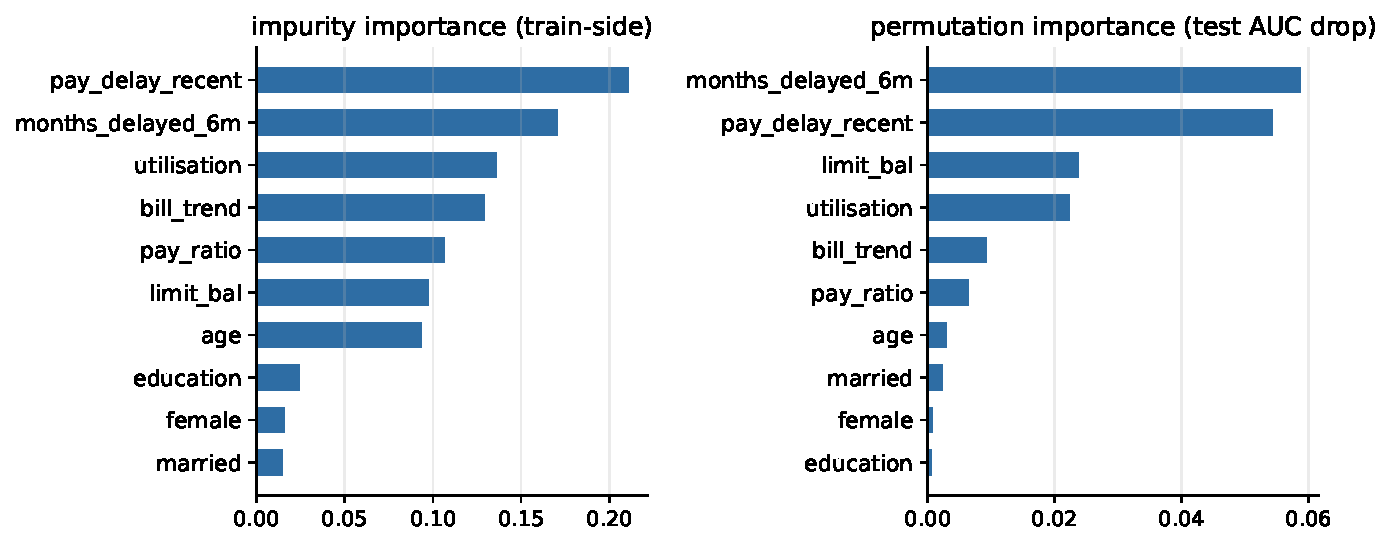
\includegraphics[width=0.88\textwidth]{figures/fig_importance.pdf}
  \end{center}
  \begin{itemize}\small
    \item \textbf{Impurity importance} (left): how much Gini each feature
          removed - free, train-side, and \alert{biased} (loves
          high-cardinality features; splits credit among correlated ones).
    \item \textbf{Permutation importance} (right): shuffle one column on the
          \emph{test set}, measure the AUC drop - slower, model-agnostic,
          honest about what the model \emph{uses}.
  \end{itemize}
\end{frame}

% ---------------------------------------------------------------
\begin{frame}{SHAP in one slide}
  \begin{itemize}
    \item Remember Block 2's receipt - each feature's exact contribution
          to one customer's log-odds? For logistic regression that
          decomposition is free.
    \item \alert{SHAP} generalises the receipt to any model: for one
          prediction, attribute the deviation from the average outcome
          across features, fairly (Shapley values, from game theory).
    \item Local: one customer's bars (adverse-action material). Global:
          average $|$contribution$|$ = an importance ranking with
          direction.
    \item Costs and caveats: computation; correlated features share credit
          ambiguously; and it explains \alert{the model}, not the world.
  \end{itemize}
  \vspace{0.4em}
  \begin{center}\small
    Lab: permutation importance today; curious? \texttt{pip install shap}
    and point it at your tournament winner at home.
  \end{center}
\end{frame}

% ---------------------------------------------------------------
\begin{frame}{Domain knowledge as a constraint: monotonicity}
  \begin{itemize}
    \item Credit intuition: risk should not \emph{decrease} as utilisation
          rises. But an unconstrained tree ensemble can produce local
          \alert{dips} - artefacts of noise.
    \item Modern GBDT accepts \alert{monotonic constraints}: force the
          score to be non-decreasing in chosen features
          (\texttt{monotonic\_cst} in sklearn).
    \item Three birds, one stone: regularisation (fewer wiggles),
          explainability (no ``more debt, less risk'' surprises), and
          regulator comfort.
    \item The same move as Block 1's binning and Block 2's coefficients:
          \emph{domain knowledge entering the model on purpose}.
  \end{itemize}
\end{frame}

% ---------------------------------------------------------------
\begin{frame}{Explanations explain the model - not the world}
  \begin{itemize}
    \item Importance $\ne$ causality: utilisation ``mattering'' means the
          \emph{model} leans on it, not that reducing it lowers risk.
    \item Correlated features trade places freely between runs -
          remember the lasso picking one twin (Block 2).
    \item Legitimate uses: \alert{debugging} (a dominant weird feature =
          leakage smell), \alert{monitoring} (importance drift),
          \alert{communication} (with the caveats spoken aloud).
    \item Policy conclusions need causal designs - beyond this course,
          but not beyond your career.
  \end{itemize}
\end{frame}

% ============================================================
% SECTION: LAB
% ============================================================
\section{Lab}

% ---------------------------------------------------------------
\begin{frame}[plain]
  \begin{center}
    \vspace{1.5cm}
    {\LARGE\textbf{Laboratory}}\\[0.6cm]
    {\normalsize Notebook \texttt{03\_trees\_ensembles\_evaluation} - laptops out.}
  \end{center}
\end{frame}

% ---------------------------------------------------------------
\begin{frame}{Lab today}
  \begin{columns}[T]
    \begin{column}{0.54\textwidth}
      \textbf{Notebook \texttt{03\_trees\_ensembles\_evaluation}}
      \begin{itemize}\small
        \item cross-validate the Block 2 baseline
        \item grow a tree, read it, leash it
        \item run the tournament: tree vs RF vs GBDT
        \item ROC, PR, calibration on the winner
        \item \alert{detonate the leak} yourselves
        \item expected cost: pick the threshold
      \end{itemize}
    \end{column}
    \begin{column}{0.44\textwidth}
      \textbf{Done =}
      \begin{itemize}\small
        \item you can say \emph{which model won, by how much, and whether
              the gap beats the CV spread}
        \item you can name \emph{your} threshold and defend it with a cost
              curve
      \end{itemize}
      \vspace{0.4em}
      \textbf{Optional extras}
      \begin{itemize}\small
        \item feed raw NaNs to HistGBDT
        \item monotonic constraints
      \end{itemize}
    \end{column}
  \end{columns}
\end{frame}

% ============================================================
% SECTION: SUMMARY
% ============================================================
\section{Summary}

% ---------------------------------------------------------------
\begin{frame}[plain]
  \begin{center}
    \vspace{1.5cm}
    {\LARGE\textbf{Summary}}\\[0.6cm]
    {\normalsize What to take home from Block 3.}
  \end{center}
\end{frame}

% ---------------------------------------------------------------
\begin{frame}{Block 3 in five sentences}
  \begin{enumerate}
    \item Trees turn data into \textbf{rules}, find interactions natively,
          and are too nervous to work alone.
    \item Ensembles manufacture disagreement - \textbf{bagging} calms
          variance, \textbf{boosting} chips at bias - and every leash is
          still the U-curve.
    \item Judge models by \textbf{CV mean $\pm$ spread}; judge rankings by
          \textbf{AUC/Gini}, rare positives by \textbf{PR}, probabilities by
          \textbf{calibration}, decisions by \textbf{expected cost}.
    \item \textbf{Leakage} makes models look brilliant precisely because
          every metric is its accomplice - only feature reasoning and
          out-of-time tests catch it.
    \item Complexity must \textbf{earn its keep} against a baseline -
          and on the real portfolio it pays at every rung, about +4 AUC
          points end to end.
  \end{enumerate}
\end{frame}

% ---------------------------------------------------------------
\begin{frame}{Project status \& reminder - topics locked today}
  \begin{itemize}
    \item \alert{Topic descriptions were due at 17:10 today.} Teams and
          topics are now final - from here on, you build.
    \item You now own both required model families: a linear baseline and a
          tree ensemble. The rubric's evaluation criterion (20\%) reads:
          \emph{``correct, leakage-aware''} - today defined both words.
    \item Minimum evaluation kit for the project: CV mean $\pm$ sd,
          ROC/AUC \emph{and} PR, a calibration look, one cost-based
          threshold argument, and a written time-travel audit of your
          features.
  \end{itemize}
  \vspace{0.5em}
  \begin{center}\small
    That kit, executed cleanly, is most of the difference between a passing
    project and a memorable one.
  \end{center}
\end{frame}

% ---------------------------------------------------------------
\begin{frame}{Exam practice - multiple choice}
  \small
  \textbf{Q1.} A risk report states ``Gini = 0.55''. This refers to:
  \begin{enumerate}[(a)]
    \item the Gini impurity used to choose tree splits
    \item the ranking metric $2\cdot\text{AUC}-1$
    \item the share of defaults in the portfolio
    \item the depth of the decision tree
  \end{enumerate}
  \vspace{0.4em}
  \textbf{Q2.} Model A: CV AUC $0.745 \pm 0.010$. Model B: $0.752 \pm 0.011$,
  same folds. The honest conclusion:
  \begin{enumerate}[(a)]
    \item B wins - deploy it
    \item the gap is within the fold spread - not yet evidence of a real difference
    \item A wins - it has the smaller spread
    \item cross-validation cannot compare models
  \end{enumerate}
\end{frame}
% Answer key: Q1 (b) - same statistician, different formula; impurity lives
% inside trees, the coefficient lives in evaluation. Q2 (b) - a difference
% of ~0.007 against a spread of ~0.010 is sampling noise until proven
% otherwise; more folds/data or a paired test before any deployment claim.

% ---------------------------------------------------------------
\begin{frame}{Exam practice - open question}
  \begin{block}{In the style of the term-0 exam ($\sim$60\% open questions)}
    A colleague adds one feature to the PD model and test AUC jumps from
    0.77 to 0.95. They propose shipping it. What do you suspect, which two
    checks do you run, and what makes this failure mode dangerous?
  \end{block}
  \vspace{0.5em}
  \begin{center}\small
    4-6 sentences. ``Too good to be true'' is the start of the answer,
    not the end.
  \end{center}
\end{frame}
% A good answer: suspect leakage. Check 1 - the time-travel test: could this
% feature's value be known at application time, for every row? Check 2 -
% out-of-time validation and a look at what importance crowns. Dangerous
% because every metric is the leak's accomplice: CV, the test set and
% importance all reward it, so no number raises the alarm - only feature
% reasoning does. Behavioural PD models live near Gini 0.5-0.7; 0.9 is a
% subpoena, not a triumph.

% ---------------------------------------------------------------
\begin{frame}[plain]
  \begin{center}
    \vspace{1.5cm}
    {\LARGE\textbf{Next week: clustering \& dimensionality reduction.}}\\[0.6cm]
    {\normalsize No labels. New questions.}
  \end{center}
\end{frame}

% ---------------------------------------------------------------
\begin{frame}{Keep learning - Block 3 reading}
  \begin{itemize}
    \item \textbf{Breiman} - \emph{Random Forests} (Machine Learning, 2001)
          - the original forest paper: bagging, OOB and importance from
          the source.
    \item \textbf{Fawcett} - \emph{An Introduction to ROC Analysis}
          (Pattern Recognition Letters, 2006) - the standard ROC/AUC paper,
          very readable.
    \item \textbf{Kaufman, Rosset \& Perlich} - \emph{Leakage in Data
          Mining} (KDD 2011) - a bestiary of real leaks; today's detonation,
          industrialised.
    \item \textbf{scikit-learn User Guide} - \emph{Model evaluation}
          section: every metric we used, with the fine print.
  \end{itemize}
\end{frame}

\end{document}
